%%%%%%%%%%%%%%%%%%%%%%%%%%%%%%%%%%%%%%%%%
% Beamer Presentation
% LaTeX Template
% Version 1.0 (10/11/12)
%
% This template has been downloaded from:
% http://www.LaTeXTemplates.com
%
% License:
% CC BY-NC-SA 3.0 (http://creativecommons.org/licenses/by-nc-sa/3.0/)
%
%%%%%%%%%%%%%%%%%%%%%%%%%%%%%%%%%%%%%%%%%

%----------------------------------------------------------------------------------------
%	PACKAGES AND THEMES
%----------------------------------------------------------------------------------------

\documentclass[aspectratio=169]{beamer}

\mode<presentation> {

% The Beamer class comes with a number of default slide themes
% which change the colors and layouts of slides. Below this is a list
% of all the themes, uncomment each in turn to see what they look like.

%\usetheme{default}
%\usetheme{AnnArbor}
%\usetheme{Antibes}
%\usetheme{Bergen}
%\usetheme{Berkeley}
\usetheme{Berlin}
%\usetheme{Boadilla}
%\usetheme{CambridgeUS}
%\usetheme{Copenhagen}
%\usetheme{Darmstadt}
%\usetheme{Dresden}
%\usetheme{Frankfurt}
%\usetheme{Goettingen}
%\usetheme{Hannover}
%\usetheme{Ilmenau}
%\usetheme{JuanLesPins}
%\usetheme{Luebeck}
%\usetheme{Madrid}
%\usetheme{Malmoe}
%\usetheme{Marburg}
%\usetheme{Montpellier}
%\usetheme{PaloAlto}
%\usetheme{Pittsburgh}
%\usetheme{Rochester}
%\usetheme{Singapore}
%\usetheme{Szeged}
%\usetheme{Warsaw}

% As well as themes, the Beamer class has a number of color themes
% for any slide theme. Uncomment each of these in turn to see how it
% changes the colors of your current slide theme.

%\usecolortheme{albatross}
%\usecolortheme{beaver}
%\usecolortheme{beetle}
%\usecolortheme{crane}
%\usecolortheme{dolphin}
%\usecolortheme{dove}
%\usecolortheme{fly}
%\usecolortheme{lily}
%\usecolortheme{orchid}
%\usecolortheme{rose}
%\usecolortheme{seagull}
%\usecolortheme{seahorse}
%\usecolortheme{whale}
%\usecolortheme{wolverine}

%\setbeamertemplate{footline} % To remove the footer line in all slides uncomment this line
%\setbeamertemplate{footline}[page number] % To replace the footer line in all slides with a simple slide count uncomment this line

%\setbeamertemplate{navigation symbols}{} % To remove the navigation symbols from the bottom of all slides uncomment this line
}

\usepackage{graphicx} % Allows including images
\usepackage{booktabs} % Allows the use of \toprule, \midrule and \bottomrule in tables

%----------------------------------------------------------------------------------------
%	TITLE PAGE
%----------------------------------------------------------------------------------------

\title[Subset selection with chance constraints ]{A practical approach to subset selection with chance constraints } % The short title appears at the bottom of every slide, the full title is only on the title page

\author[Monks \& Currie]{Thomas Monks \inst{1} \and Christine S.M Currie \inst{2}}
\institute[University of Southampton]{\inst{1} NIHR CLAHRC Wessex, UoS / Alan Turing Institute \and \inst{2} CORMSIS, University of Southampton  }


\date{Winter Simulation Conference 2018}%Date, can be changed to a custom date

\begin{document}

\begin{frame}
\titlepage % Print the title page as the first slide
\end{frame}

\begin{frame}
\frametitle{Overview} % Table of contents slide, comment this block out to remove it
\tableofcontents % Throughout your presentation, if you choose to use \section{} and \subsection{} commands, these will automatically be printed on this slide as an overview of your presentation
\end{frame}

%----------------------------------------------------------------------------------------
%	PRESENTATION SLIDES
%----------------------------------------------------------------------------------------

%------------------------------------------------
\section{Problem description} %------------------------------------------------

\subsection{Motivation} % A subsection can be created just before a set of slides with a common theme to further break down your presentation into chunks


\begin{frame}
\frametitle{Motivation}
\textbf{Aim}: support system experts making complex decisions involving \textbf{multiple objectives} and a \textbf{large number of scenarios} for the system\\
\textbf{Factors}:
\begin{itemize}
\item Some unquantifiable (e.g., political) variables 
\item Large, complex, slow-running simulation model 
\item Simulation practitioner without a PhD in statistics/simulation
\item Off-the-shelf simulation package 
\end{itemize}
\end{frame}

%------------------------------------------------

\begin{frame}
\frametitle{Motivation}
\textbf{Aim}: support system experts making complex decisions involving \textbf{multiple objectives} and a \textbf{large number of scenarios} for the system\\
\textbf{Factors}:
\begin{itemize}
\item Some unquantifiable (e.g., political) variables:   \textcolor{red}{Find a subset not a single optimum}
\item Large, complex, slow-running simulation model:  \textcolor{red}{Use variance reduction techniques, e.g., CRN}
\item Simulation practitioner without a PhD in statistics/simulation: \textcolor{red}{Reduce the need for expert statistical judgment}
\item Off-the-shelf simulation package:  \textcolor{red}{Difficult to implement fully sequential methods}
\end{itemize}
\end{frame}

%------------------------------------------------

%------------------------------------------------


\begin{frame}
\frametitle{Motivation}
\begin{block}{Requirements}
\begin{itemize}
\item[R1] The choice of options to include in the experimentation and the number of replications to make can only be changed once during the experiment (two-stage method)
\item[R2]The procedure should not impose any distributional assumptions on the simulation output

\end{itemize}
\end{block}

\end{frame}

\begin{frame}{Problem Description}
Assume that we are comparing $k\geq 2$ systems and are primarily interested in minimizing the mean value of a particular output
\[
x_{i} = \sum_{j=1}^{n}x_{ij}/n
\]
where $i=1, \ldots, k$ but are also interested in $L$ secondary outputs or objectives
\[
y_{il} = \sum_{j=1}^{n}Y_{ijl}/n
\]
\end{frame}
\begin{frame}{Subset Selection with Chance Constraints}
    \textbf{Aim:} Identify a shortlist (subset) of systems ($\mathbf{S}^{*}$) that are all within a \textbf{proportion} $\beta$ of the best system with probability $1-\alpha$
    
    \textbf{And} satisfy the chance constraints with a probability $1-\gamma$
    \vspace{1cm}
    
    We restrict the number of systems on the shortlist to $\min \{m,\vert S^{*} \vert \}$ by taking the \textbf{top} $\mathbf{m}$ systems that satisfy the above constraints 
\end{frame}

\subsection{Previous Work}
\begin{frame}{Previous Work}
\begin{enumerate}
    \item \textbf{Approach:} \cite{Branke:MS2007} suggest three categories: indifference zone, OCBA and Expected Value of Information
    \item \textbf{Chance constraints} \cite{Hong:IJOC2015} suggest two approaches to dealing with chance constraints: Expectation Constrained Selection and Chance Constrained Selection. 
    \item \textbf{Subset selection} authors use either OCBA or indifference zone methods to maximize/guarantee the probability of correct selection of the best $m$ of $k$ systems
\end{enumerate}
\end{frame}
%------------------------------------------------
\section{Methods}
\subsection{Methods}
\begin{frame}{Big Picture}
\begin{columns}[c] % The "c" option specifies centered vertical alignment while the "t" option is used for top vertical alignment

\column{.5\textwidth} % Left column and width
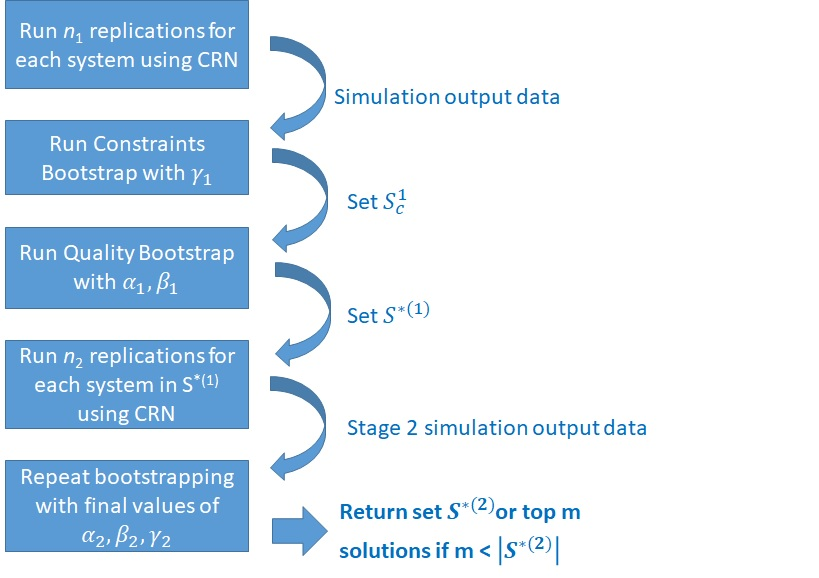
\includegraphics[width=1.2\linewidth]{Overall_Process}

\column{.45\textwidth} % Right 
\begin{itemize}
\item Method relies on bootstrapping
\item Set stage 1 parameters so that we are risk averse
\item Balancing risk of missing a good solution versus including too many in stage 2
\item Trade off between $n_{1}$ and $n_{2}$
\end{itemize}

\end{columns}


\end{frame}
\begin{frame}{Non-Parametric Bootstrapping}
Resampling method used to infer properties for a set of data.
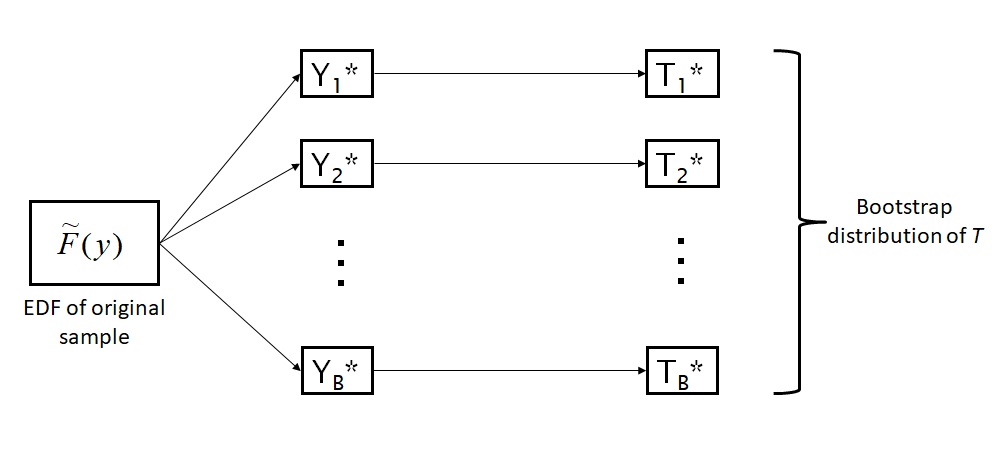
\includegraphics[width=1.0\linewidth]{Bootstrap_Diagram.jpg}
\end{frame}
\begin{frame}{Constraints Bootstrap}
\textbf{Aim:} Identify systems likely to violate the chance constraints
\begin{block}{Constraints Bootstrap}
\begin{enumerate}
    \item Input a set of bootstrap samples $\mathbf{Y}^{\star (1)}, \mathbf{Y}^{\star (2)}, \ldots, \mathbf{Y}^{\star (B)}$ and for each  calculate $y^{\star (b)}_{l}$, $l=1, \ldots, L$.
    \item Include systems in the final feasible set $\mathbf{S}_{c}$ if 
\[
\frac{1}{B} \sum_{b=1}^{B} \prod_{l=1}^{L} I \left\{ y^{\star (b)}_{l} \geq 0\right\} \geq 1-\gamma,
\]
\item Return $\mathbf{S}_{c}$.
\end{enumerate}
\end{block}
\end{frame}
\begin{frame}{Quality Bootstrap}
\textbf{Aim:} identify a set of systems with means within a distance $\beta$ of the best system with probability $1-\alpha$
\begin{block}{Quality Bootstrap}
\begin{enumerate}
\item Define a new variable $d_{ij} = x_{j}^{*}-x_{ij}$
\item Generate $B$ bootstraps of the $d_{ij}$
\item In each bootstrap sample, identify systems with differences less than $\beta \bar{x}^{*}$, where $\bar{x}^{*}$

\end{enumerate}
\end{block}
\end{frame}
\begin{frame}{Quality Bootstrap}
\begin{block}{Quality Bootstrap (Cont'd)}
\begin{enumerate}\setcounter{enumi}{3}
\item Identify $\mathbf{S}^{*}$ such that it is the biggest set for which
\[
\frac{1}{B} \sum_{b=1}^{B} \prod_{j \in \mathbf{S}_{c}} I\{\vert d^{\star (b)}_{ij} \vert \leq \beta \bar{x}^{*}\} \geq 1 - \alpha.
\]
\item Return $\mathbf{S}^{*}$
\end{enumerate}
\end{block}
\end{frame}
%------------------------------------------------
\section{Python Implementation}
%------------------------------------------------
\subsection{Setup} 
%------------------------------------------------

\begin{frame}
\frametitle{Advice on installation of Python}
%Uncomment the code on this slide to include your own image from the same directory as the template .TeX file.
\begin{figure}

\includegraphics[width=1.0\linewidth]{anaconda.png}
\end{figure}
https://www.anaconda.com/download/
\end{frame}

%------------------------------------------------


%------------------------------------------------

\begin{frame}
\frametitle{Code available from GitHub}
%Uncomment the code on this slide to include your own image from the same directory as the template .TeX file.
\begin{figure}
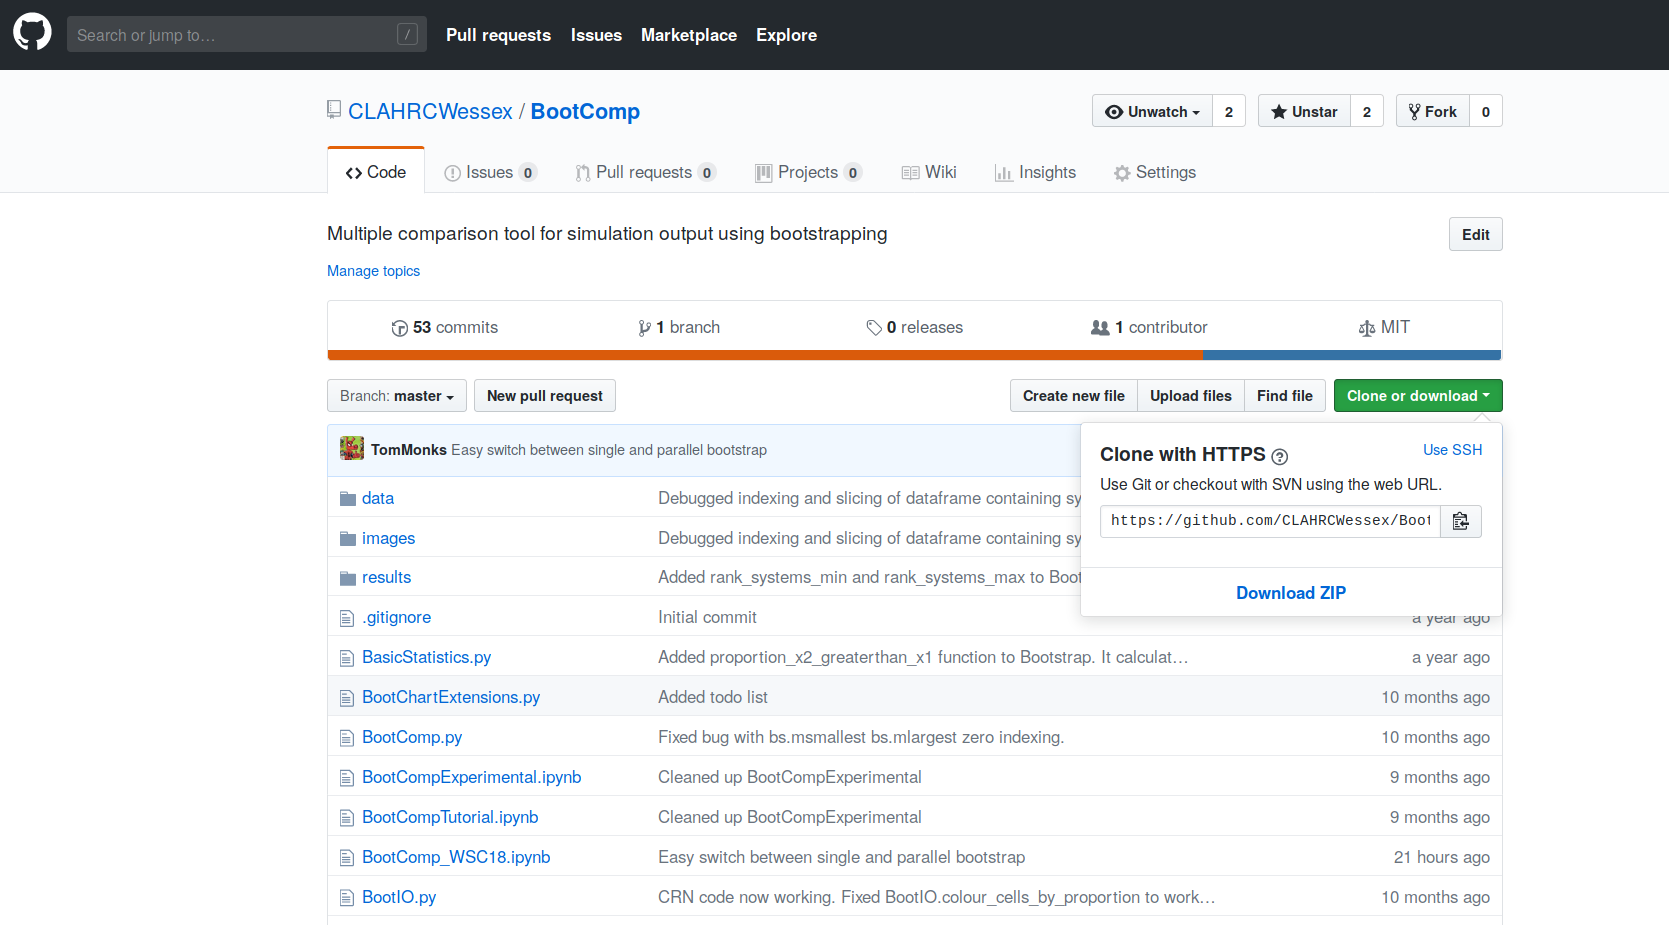
\includegraphics[width=0.95\linewidth]{github.png}
\end{figure}
https://github.com/CLAHRCWessex/BootComp
\end{frame}

%------------------------------------------------

\begin{frame}
\frametitle{Code available from GitHub}
%Uncomment the code on this slide to include your own image from the same directory as the template .TeX file.
\begin{figure}
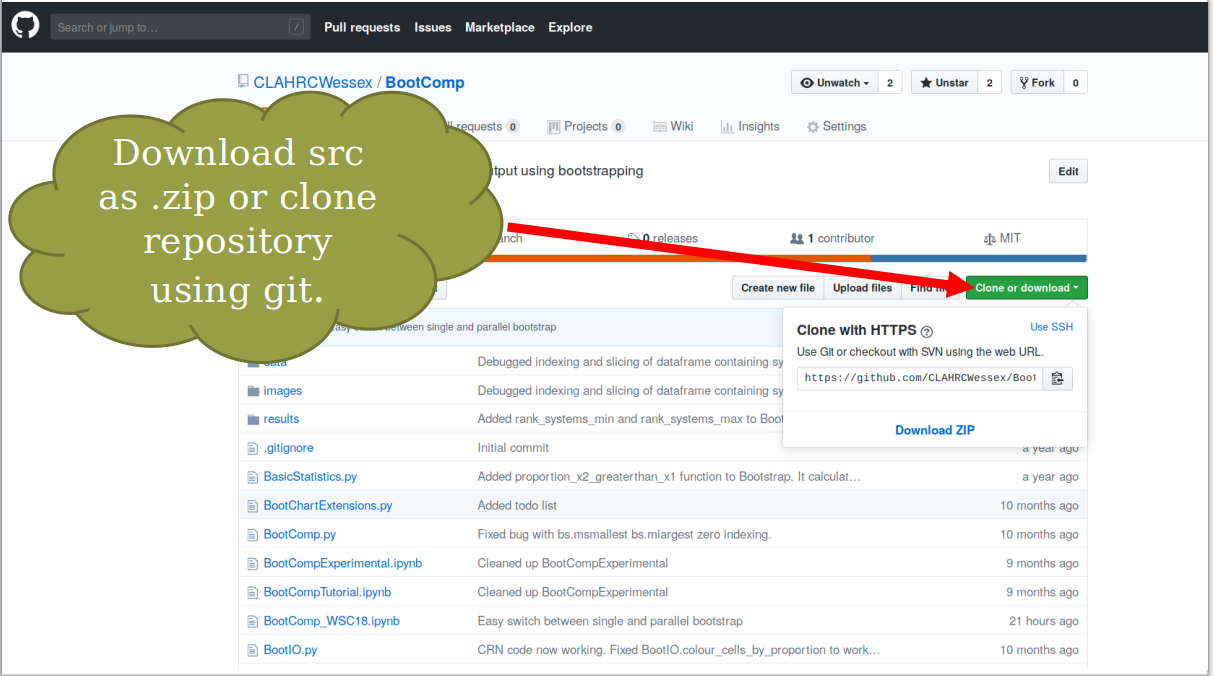
\includegraphics[width=0.95\linewidth]{github2.png}
\end{figure}
https://github.com/CLAHRCWessex/BootComp
\end{frame}

%------------------------------------------------

%------------------------------------------------

\begin{frame}
\frametitle{Jupyter Notebook Implementation}
\begin{figure}
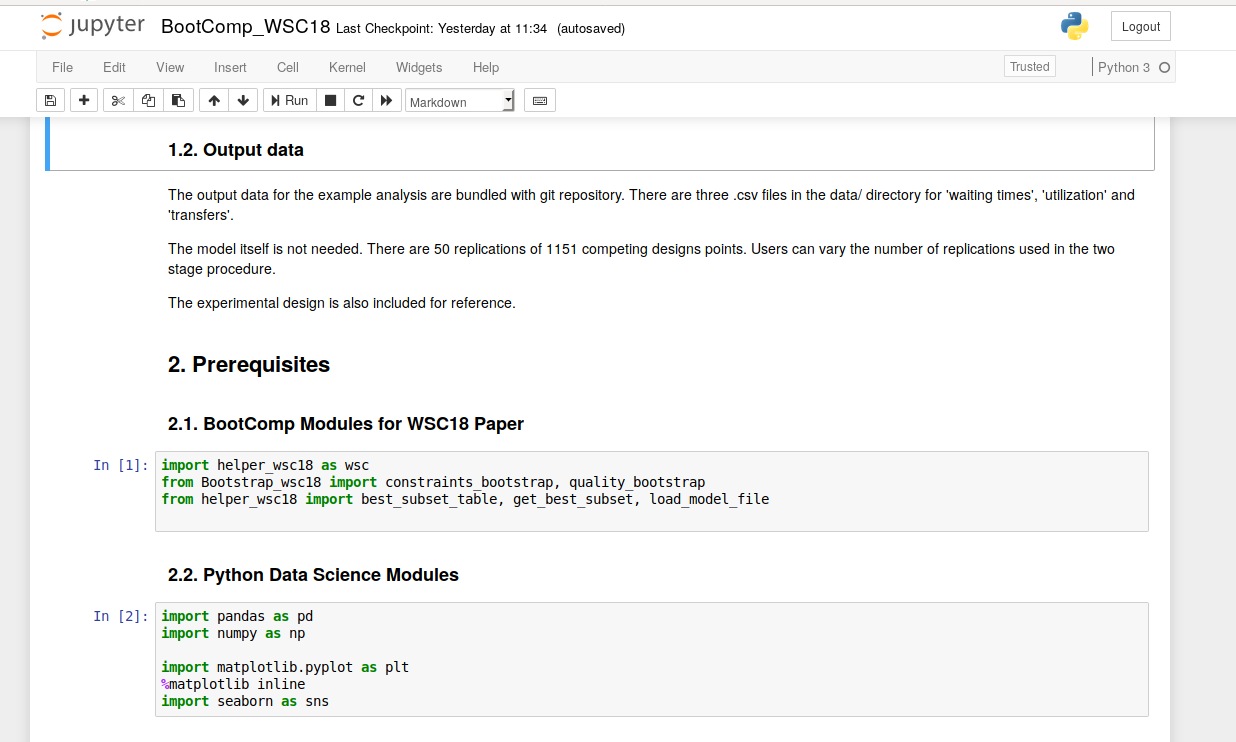
\includegraphics[width=1.0\linewidth]{juypter1.png}
\end{figure}
\end{frame}

%------------------------------------------------


\begin{frame}
\frametitle{Jupyter Notebook Implementation}
%Uncomment the code on this slide to include your own image from the same directory as the template .TeX file.
\begin{figure}
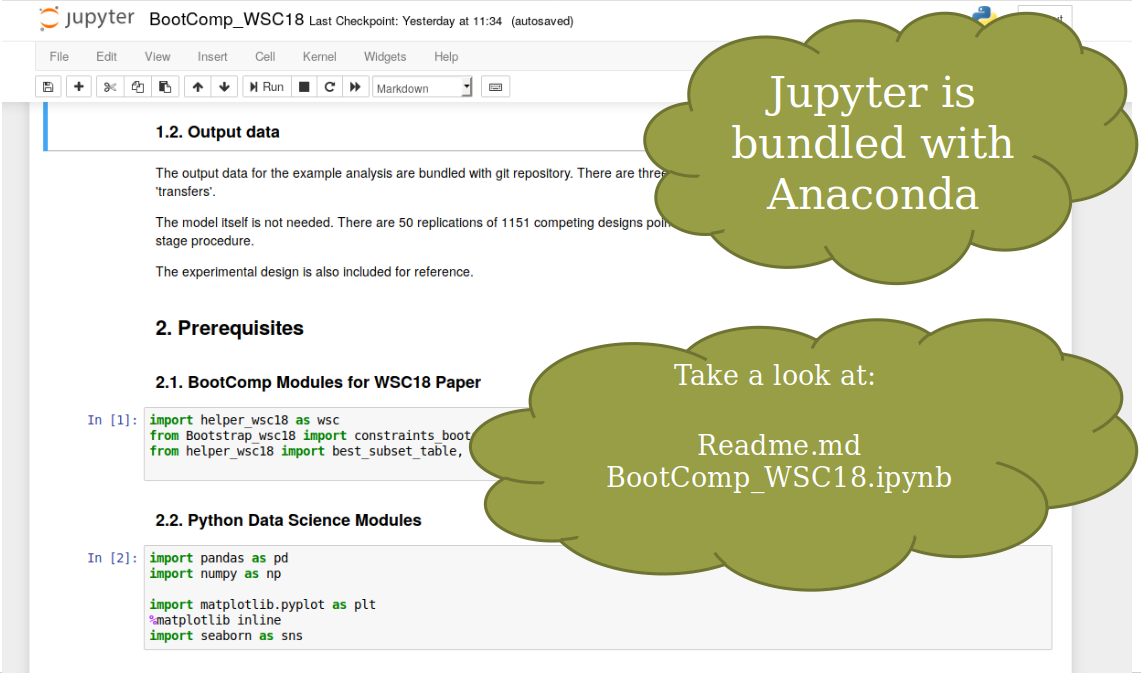
\includegraphics[width=1.0\linewidth]{jupyter2.png}
\end{figure}
\end{frame}

%------------------------------------------------

\begin{frame}[fragile]
\frametitle{Dependencies}
\begin{itemize}
\item The readme.md provides an install guide (read the readme!)
\item Create a conda environment 
\item Environments allow you to switch versions of Python packages to make sure you are using the same dependencies as the original code
\end{itemize}

\begin{verbatim}
conda env create -f environment.yml
conda activate bootcomp
\end{verbatim}

\end{frame}

%------------------------------------------------

\section{A practical problem}
\subsection{A practical problem}
\begin{frame}
\frametitle{Designing a rehabilitation ward}
%Uncomment the code on this slide to include your own image from the same directory as the template .TeX file.
\begin{figure}
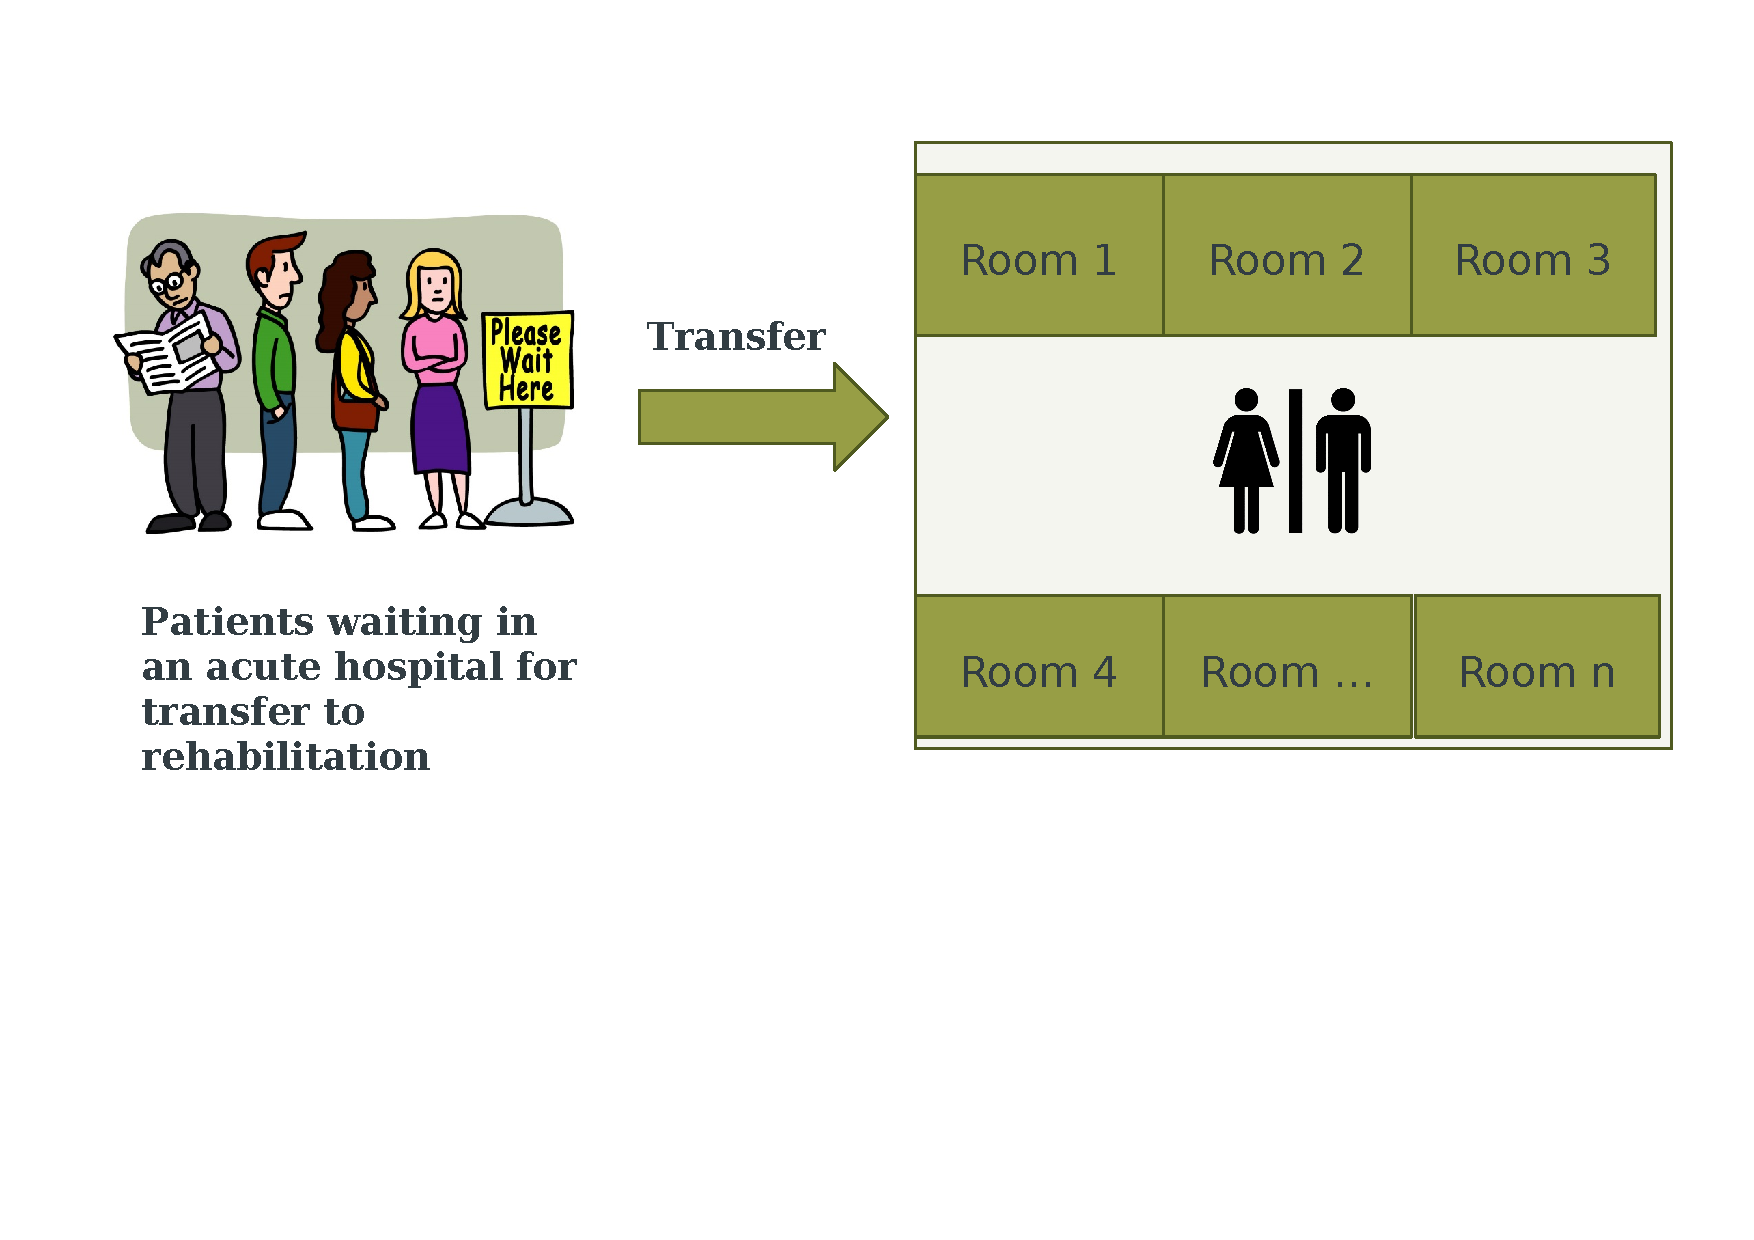
\includegraphics[width=0.95\linewidth]{ward1a.pdf}
\end{figure}
\end{frame}

%------------------------------------------------


\begin{frame}
\frametitle{Designing a rehabilitation ward}
%Uncomment the code on this slide to include your own image from the same directory as the template .TeX file.
\begin{figure}
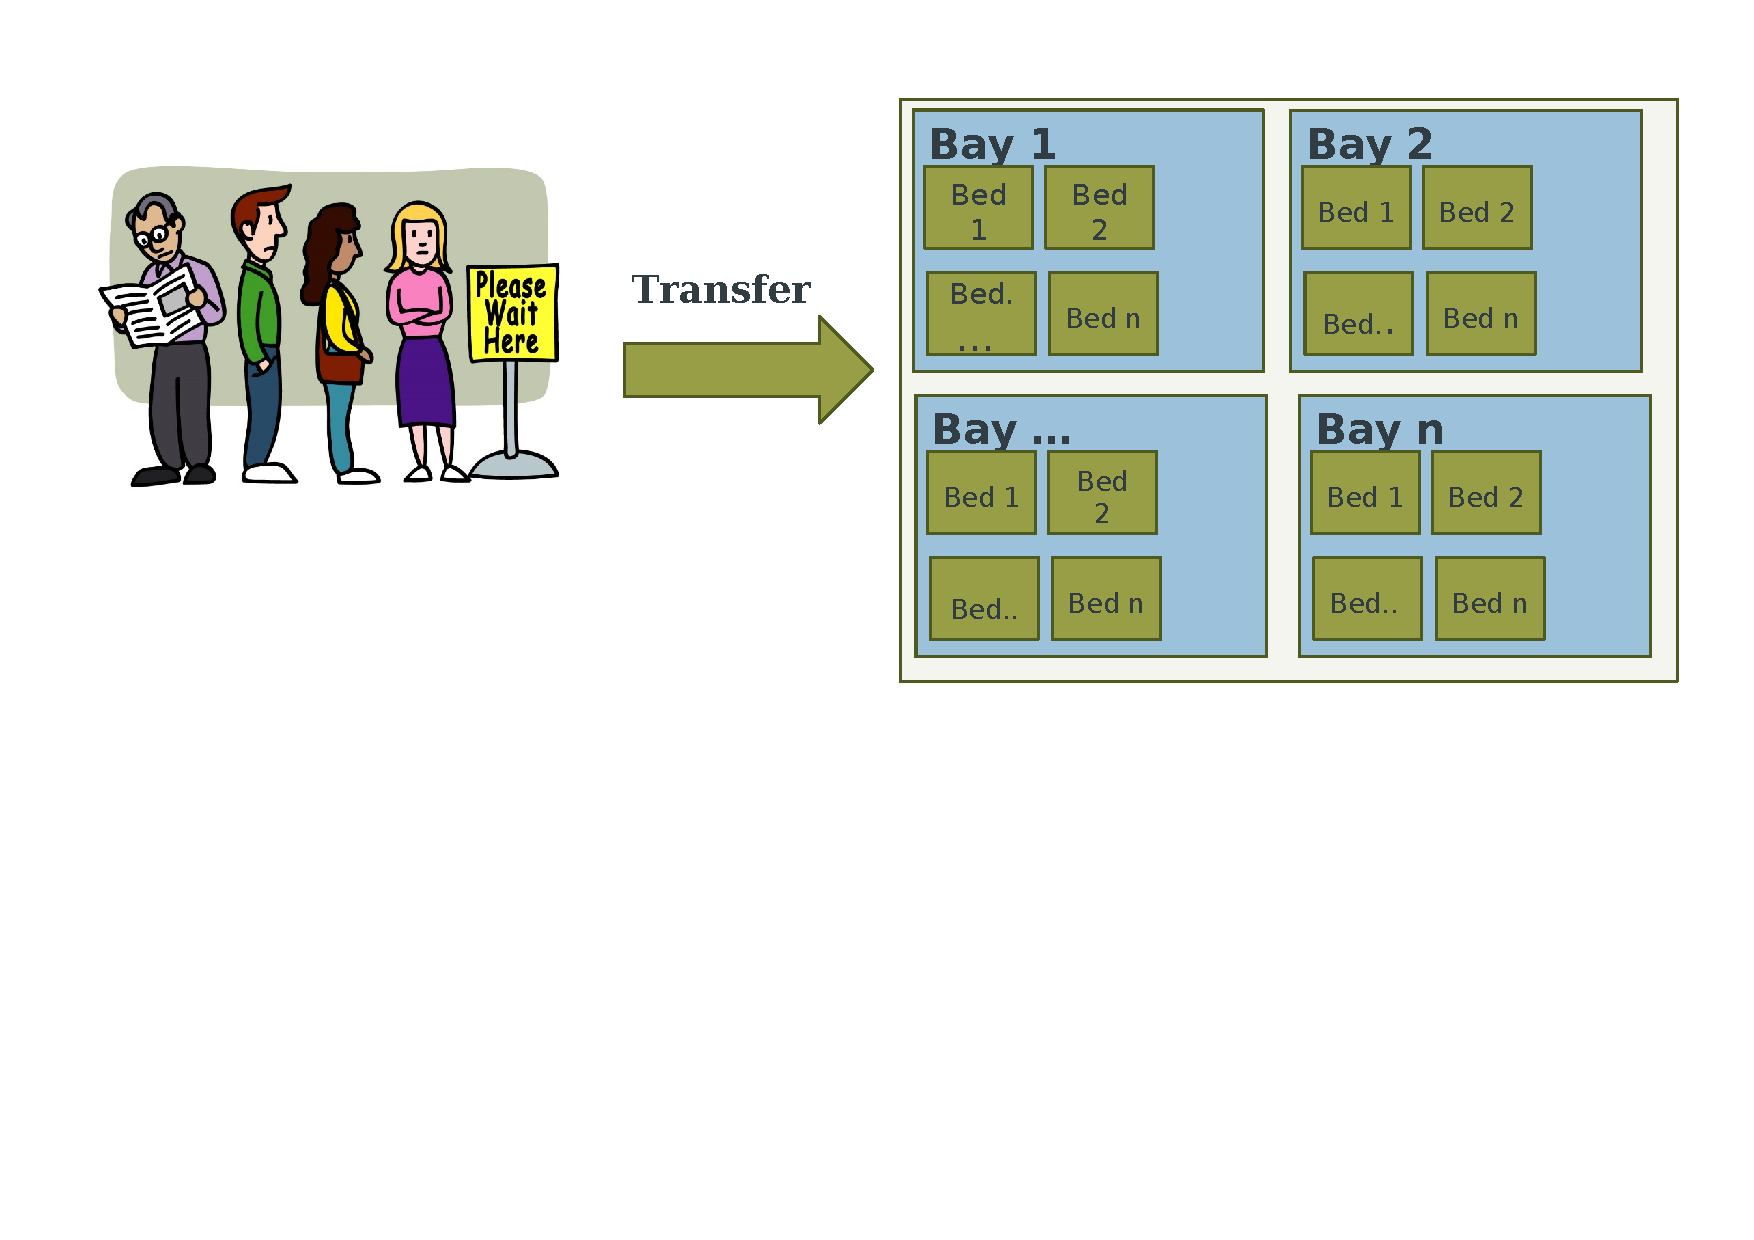
\includegraphics[width=1.0\linewidth]{ward3a.pdf}
\end{figure}
\end{frame}

%------------------------------------------------


\begin{frame}
\frametitle{Designing a rehabilitation ward}
%Uncomment the code on this slide to include your own image from the same directory as the template .TeX file.
\begin{figure}
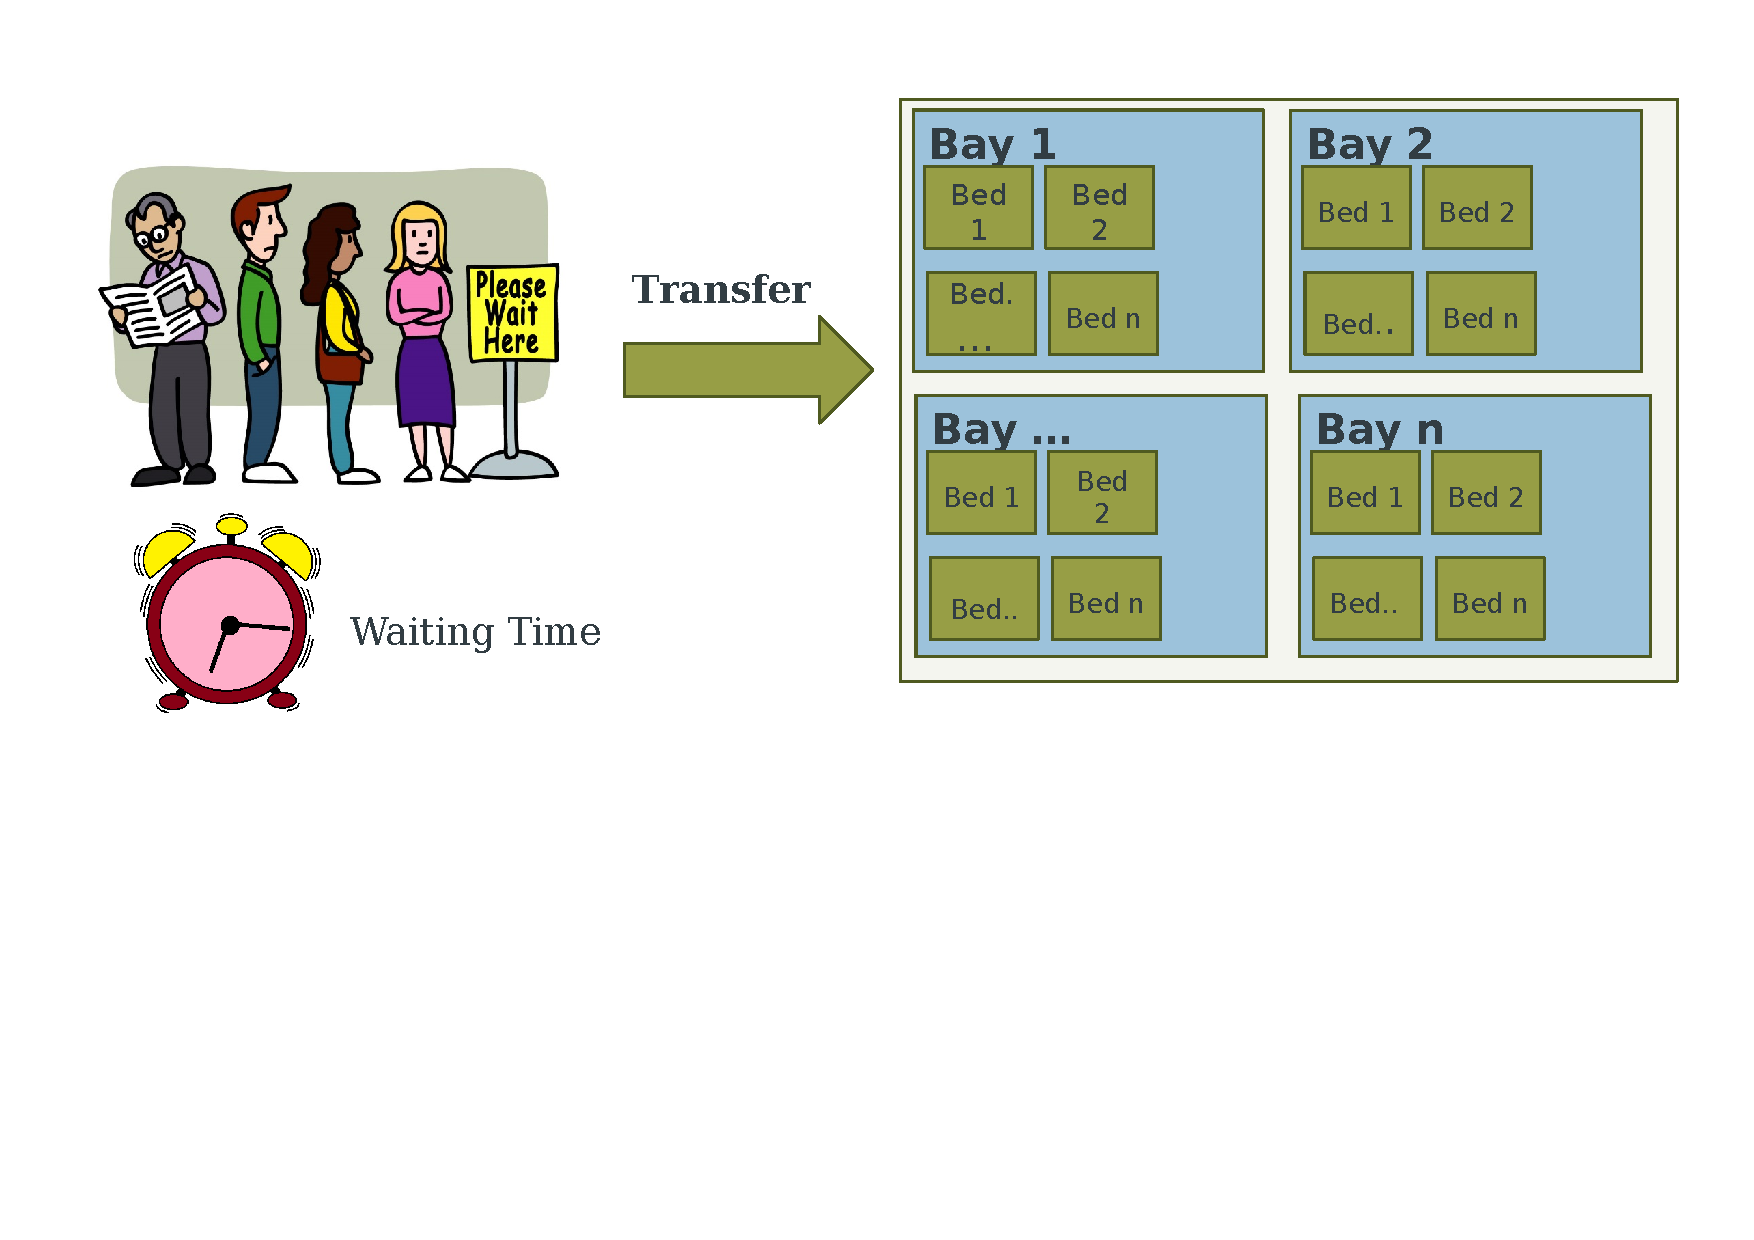
\includegraphics[width=1.0\linewidth]{ward4a.pdf}
\end{figure}
\end{frame}

%------------------------------------------------


\begin{frame}
\frametitle{Designing a rehabilitation ward}
%Uncomment the code on this slide to include your own image from the same directory as the template .TeX file.
\begin{figure}
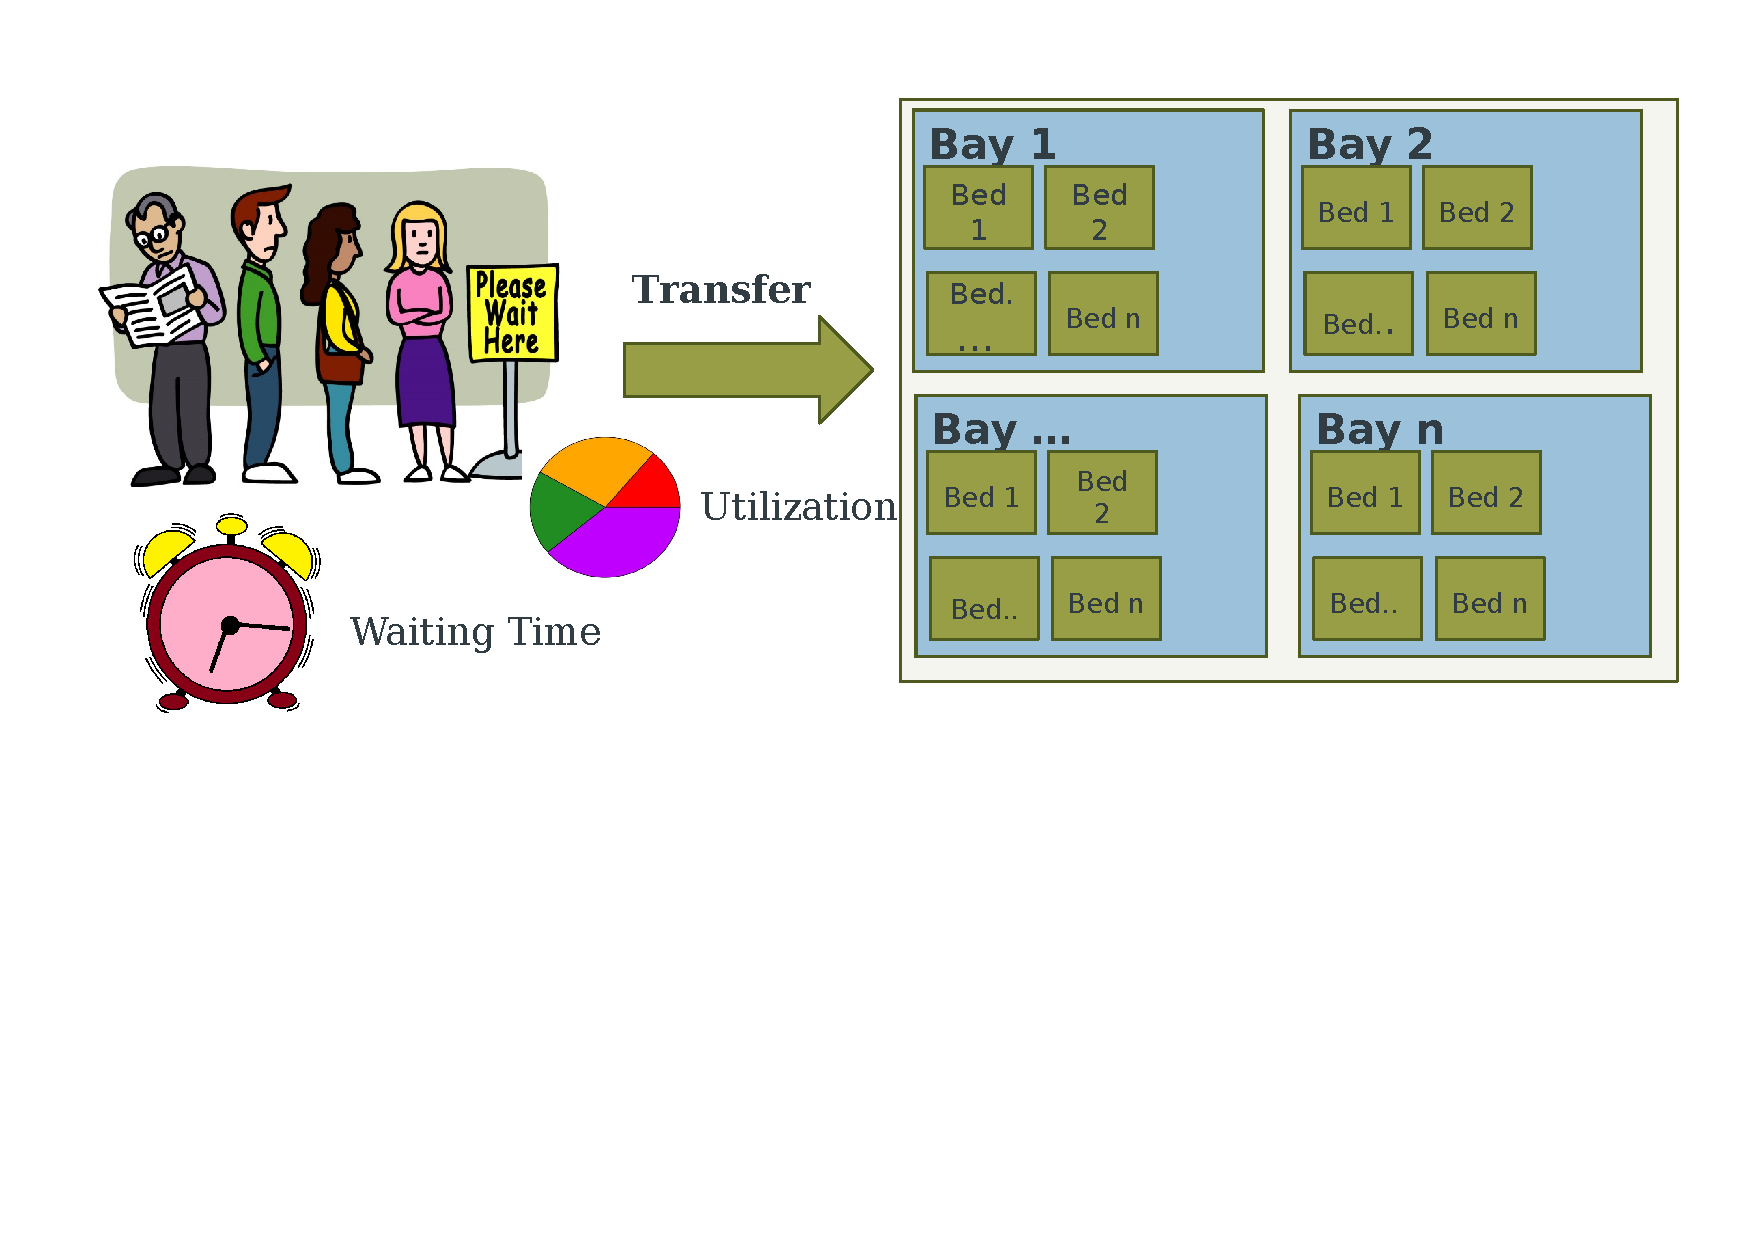
\includegraphics[width=1.0\linewidth]{ward5a.pdf}
\end{figure}
\end{frame}

%------------------------------------------------


\begin{frame}
\frametitle{Designing a rehabilitation ward}
%Uncomment the code on this slide to include your own image from the same directory as the template .TeX file.
\begin{figure}
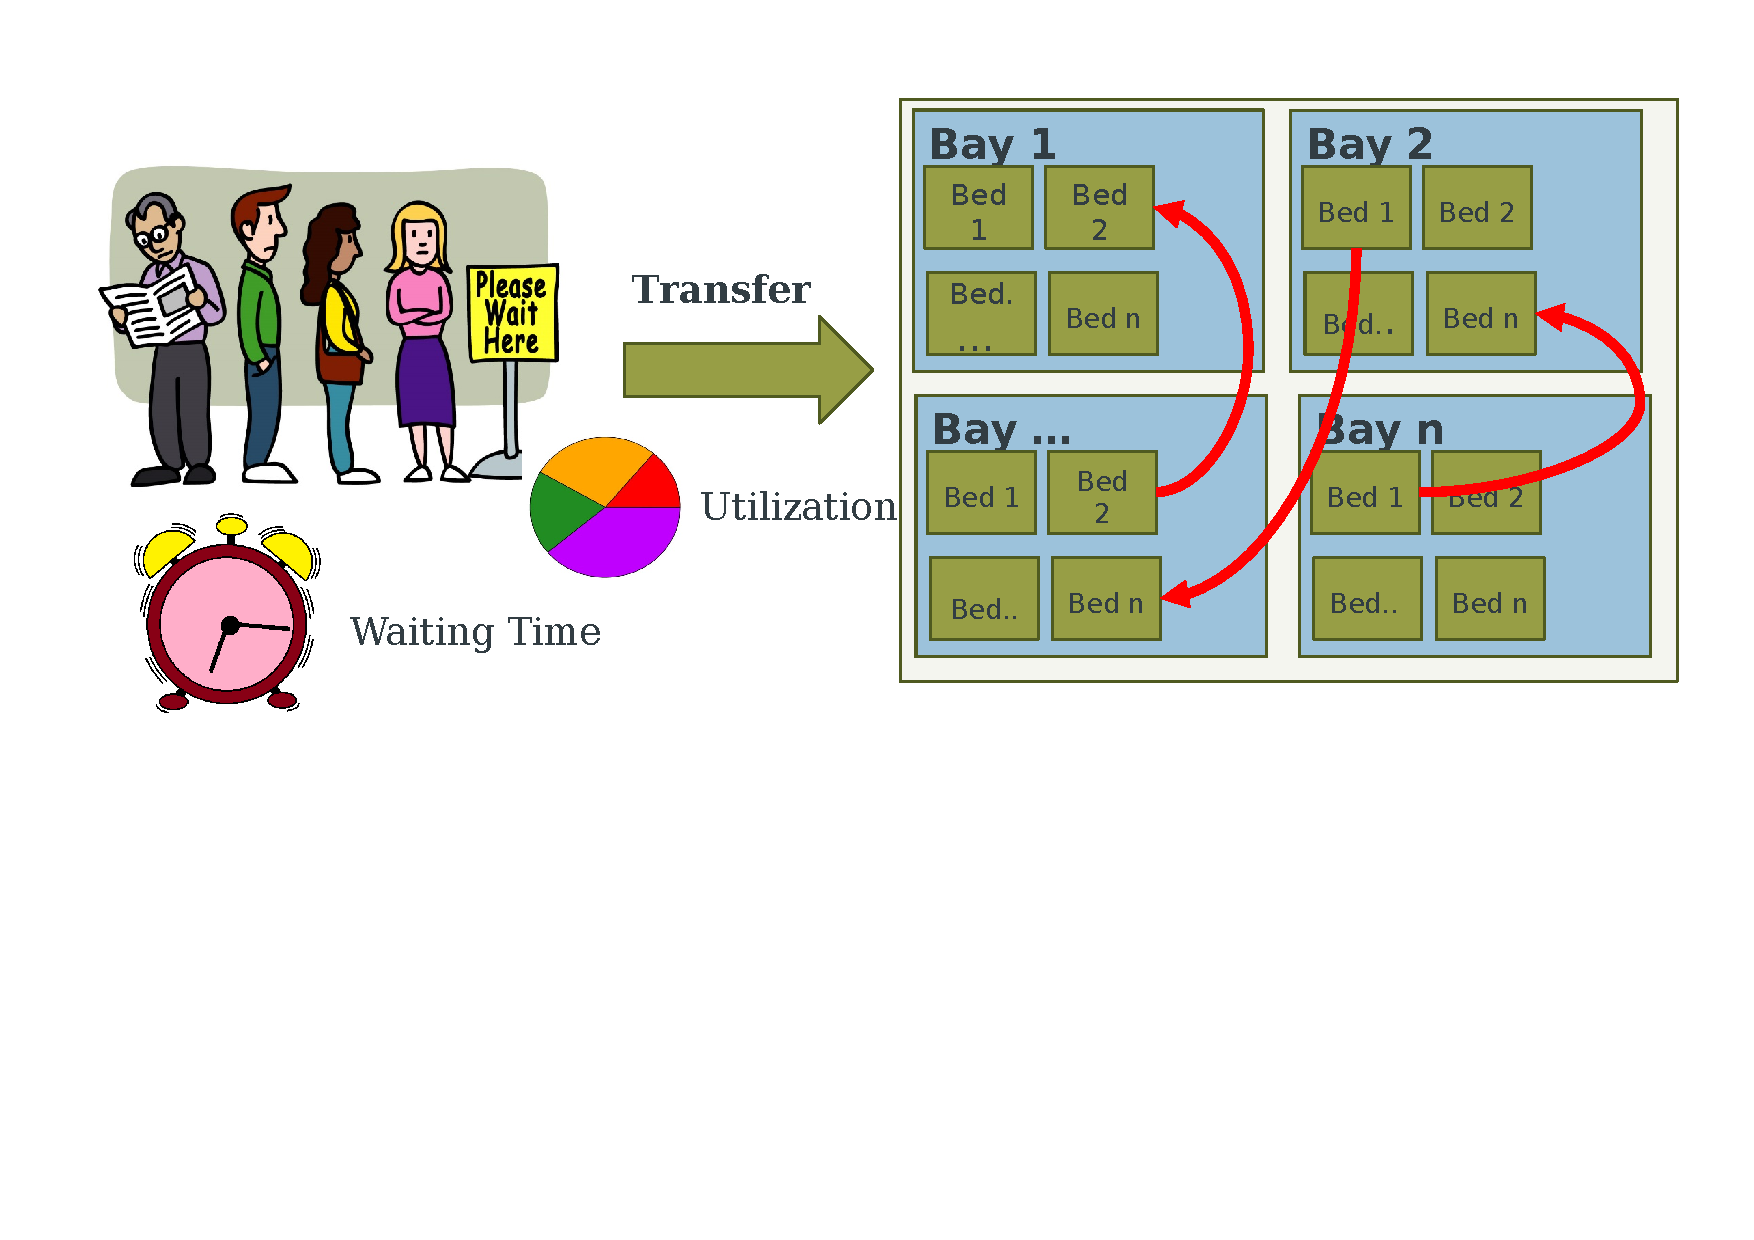
\includegraphics[width=1.0\linewidth]{ward6a.pdf}
\end{figure}
\end{frame}

%------------------------------------------------


\begin{frame}
\frametitle{Design of Experiments}

\textbf{1051 competing designs}
    \begin{block}{Decision Variables}
        \begin{itemize}
            \item No. beds 
            \item Bay size + no. bays
            \item No. single rooms  
        \end{itemize}
    \end{block}
    
    
    \begin{block}{Chance Constraints}
        \begin{itemize}
            \item Utilization of beds 
            \item Patient transfers between bays
        \end{itemize}
    \end{block}


\end{frame}

%------------------------------------------------

\begin{frame}
\frametitle{Further work}

\begin{itemize}
    \item Comparison with sequential budget allocation algorithms finding top-m systems with a \textbf{single} performance measure
    \begin{itemize}
        \item Set of 10 normal distributions $N(i,6)$
        \item Set of 100 normal distributions $Ni/100,6)$
        \item Law inventory example
    \end{itemize}
    \item Comparisons using common random numbers
    \item Identifying ``good'' values for the parameters in the first stage: $N_{0}, \alpha_{1}, \beta_{1}, \gamma_{1}$
\end{itemize}
    

\end{frame}




%------------------------------------------------



\begin{frame}
\frametitle{References}
\footnotesize{
\begin{thebibliography}{99} % Beamer does not support BibTeX so references must be inserted manually as below
\bibitem[Branke et al. 2007]{Branke:MS2007}
J\"{u}rgen Branke, Stephen E. Chick and Christian Schmidt (2007)
\newblock Selecting a selection procedure
\newblock \emph{Management Science} 53, 1916--1932

\bibitem[Hong et al. 2015]{Hong:IJOC2015} 
L. Jeff Hong, Jun Luo and Barry L. Nelson (2015)
\newblock Chance constrained selection of the best.
\newblock \emph{INFORMS Journal on Computing}
27, 317 -- 334.



\end{thebibliography}
}
\end{frame}

%------------------------------------------------
%----------------------------------------------------------------------------------------

\end{document}